\section{Architectural Design}

% Compiler
\subsection{Compiler}

The compiler follows the structure outlined in the lectures, with the additional steps that
links the resulting object code against a runtime to generate the final executable.
\begin{center}
    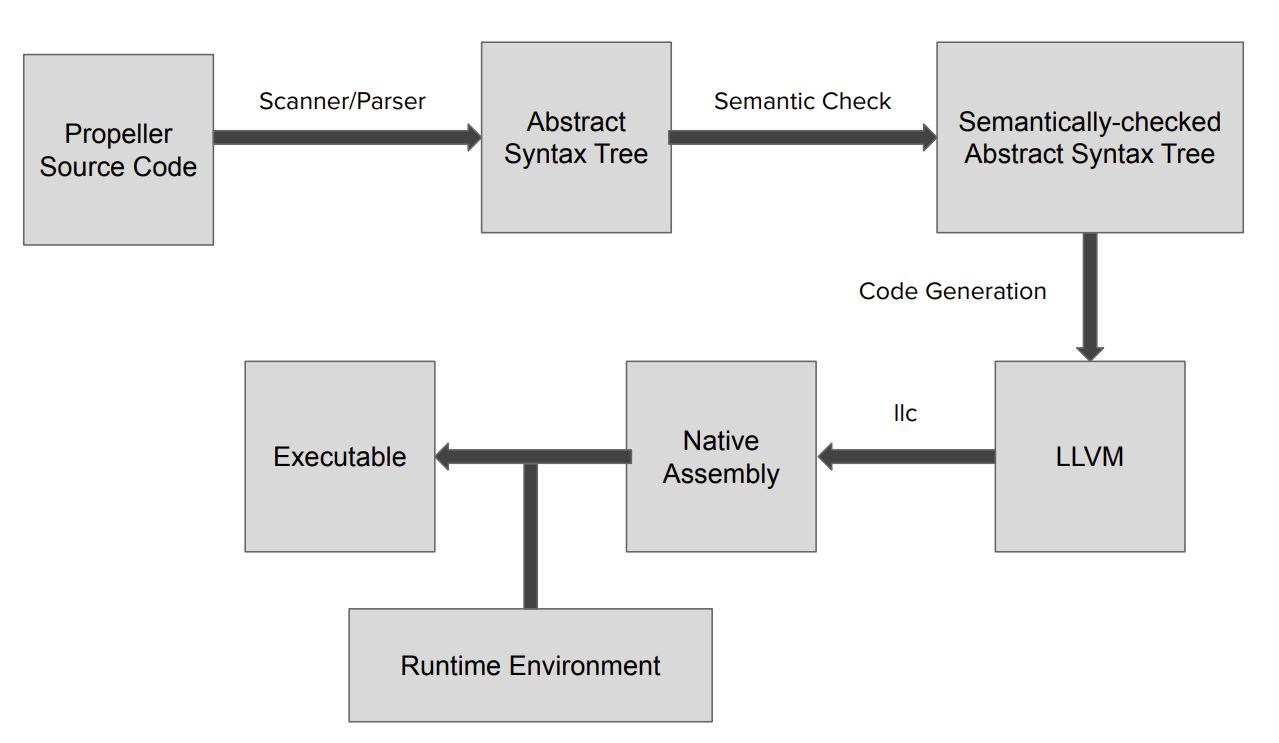
\includegraphics[scale=0.5]{block.jpg}
\end{center}

% Scanner
\subsection{Scanner}
The scanner transforms a Propeller program into a series of tokens, which are separated by
whitespace in the source code. Examples of tokens include variable names, function names,
types, separators, operators, control flow statements, and literals. Additionally, the
scanner throws a unique error if it encounters an ill-formed identifier (e.g.
\texttt{h?3\_\_llo}).

% Parser
\subsection{Parser}
The parser receives a series of tokens from the scanner, then uses these tokens to construct
an abstract syntax tree. Nothing of particular interest happens during the generation
of a Propeller program's AST.

% Semantic check
\subsection{Semantic Checker}
The semantic checker receives the AST from the parser, then performs various checks
on declarations, definitions, expressions, and statements. It prevents the programmer from
defining two or more functions with the same identifier, defining two or more
variables in the same scope with the same identifier, defining two or more object
types with the same identifier, overwriting a built-in function's definition,
using undefined identifiers, using undefined object properties, attempting to
access a property of a non-object variable, binding a function to a property
whose type does not match those of the function's formal parameters, binding a
function with some \texttt{n != 2} formal parameters to an object's property,
binding/unbinding a function to non-object variables, declaring variables of type
\texttt{void}, creating list literals of a non-primitive type, creating list
literals whose elements are of different types, passing an incorrect number of
arguments to a function, passing one or more arguments to a function whose types
does not match those of the function's formal parameters, returning a value whose
type does not match the function's return type, assigning a value to a variable
whose type differs from the value's type, and using unary and binary operators on
expressions with inappropriate types, and using \texttt{continue} or
\texttt{break} statements outside of loops. Once these checks are performed, the
semantic checker generates a semantically-checked abstract syntax tree.

% Code Generator
\subsection{Code Generator}
The code generator receives the SAST from the semantic checker, then converts
the SAST into an LLVM IR of the original Propeller program. Several additional
checks are performed as the instructions are being generated, which prevent
duplicate bindings of a function to the same property, prevent the unbinding
of a function from a property if it is not already bound, and assignment of
properties to external objects. 

\subsubsection{Bindings}
Bindings are processed in the code generation phase. It
keeps track of which functions are bound to the properties of object
variables using a single string map, which maps a combination of object
variable names and their properties to a list of function names.

% Runtime Environment
\subsection{External objects and Runtime Environment}
External objects are treated uniquely by Propeller. They are
not objects that occupy memory spaces in the Propeller module; instead, all
Propeller code treats them as integer values, like an identification for the
corresponding instance.

The sole purpose of runtime environments in Propeller is to provide
implementation of external objects. All interactions with external objects
within propeller are translated into calls to functions in the runtime
environment.

For each external object type, the runtime environment must implement\\
\verb|int object_new_<typename>()|, which creates an object of \verb|typename|
and returns its identification.

For each property of object type \verb|typename|, four functions must be
implemented:
\begin{itemize}
\item \verb|prop_t object_prop_get_<typename>_<propname>(int id)|: Gets the
value of property \verb|propname| of object with id \verb|id|. The return type
must match that of the property.
\item \verb|void object_prop_assign_<typename>_<propname>(int id, prop_t val)|:
Assign \verb|val| to the value of property \verb|propname| of object with id
\verb|id|. This is not actually implemented because we don't have a use for it
since GUI support is cancelled.
\item \verb|void object_prop_bind_<typename>_<propname>(int id, funcptr_t func)|:
Bind a function to the property \verb|propname| of object with id \verb|id|.
\verb|func| is a function in the Propeller module and is guaranteed to take two
parameters of the same type of the property.
\item \verb|void object_prop_unbind_<typename>_<propname>(int id, funcptr_t func)|:
Same as above, but unbinds the function.
\end{itemize}

Since Propeller does not have garbage collection capabilities yet, the runtime
cannot delete any of the objects it creates.

The runtime environment is required to run the entry point to the Propeller module
\verb|init()| on startup, then it can run any routine that's needed to notify the
Propeller module of changes of property values. They are usually implemented as
an ``event loop", either with polling or wait for some system calls to return.

% Work split
\subsection{Component-level work split}

\begin{itemize}
\item Lexer: Randy
\item Parser: Randy
\item Semantic Analysis:
  \begin{itemize}
  \item base SAST transformation: Randy
  \item function: Randy
  \item operators, expressions: Randy
  \item lists: Isra and Randy
  \item strings: Isra and Chris
  \item if statement: Randy
  \item while statement: Randy and Chris
  \item break and continue statement: Chris
  \item for statement: Randy
  \item return statement: Randy and Chris
  \item built-in functions: Randy and Isra
  \item objects: Randy
  \item external objects: Chris
  \item bindings: Randy
  \end{itemize}
\item Code generation:
  \begin{itemize}
    \item function: Randy
    \item return: Chris
    \item integer literals: Randy
    \item boolean literals and operators: Gwendolyn
    \item modulo operator: Chris
    \item float literals: Randy
    \item other binary and unary operators: Randy
    \item if statement: Randy
    \item while statement: Randy and Chris
    \item break and continue statement: Chris
    \item for statement: Randy
    \item list literals: Isra
    \item objects: Randy
    \item strings: Isra
    \item bindings: Randy
    \item external object bindings: Chris
    \item built-in functions: Randy, Isra and Chris
  \end{itemize}
\item Runtime: Chris
\end{itemize}
